\DiaryEntry{Groups and GAP}{2020-09-25}{Algebra}

This entry shall show how we can connect usage of GAP and the "Group Explorer" with manually calculated results.

\subsection{Symmetric Group $S_3$}

Let's start with the symmetric group $S_3$. From previous journal entries we know that this group has order $6$ and is isomorphic to the dihedral group of order six, the group of symmetries of the equilateral triangle.

From \href{https://nathancarter.github.io/group-explorer/GroupInfo.html?groupURL=https://nathancarter.github.io/group-explorer/groups/S_3.group}{Group Explorer} we obtain the following multiplication table.

\begin{figure}[H]
    \centering
    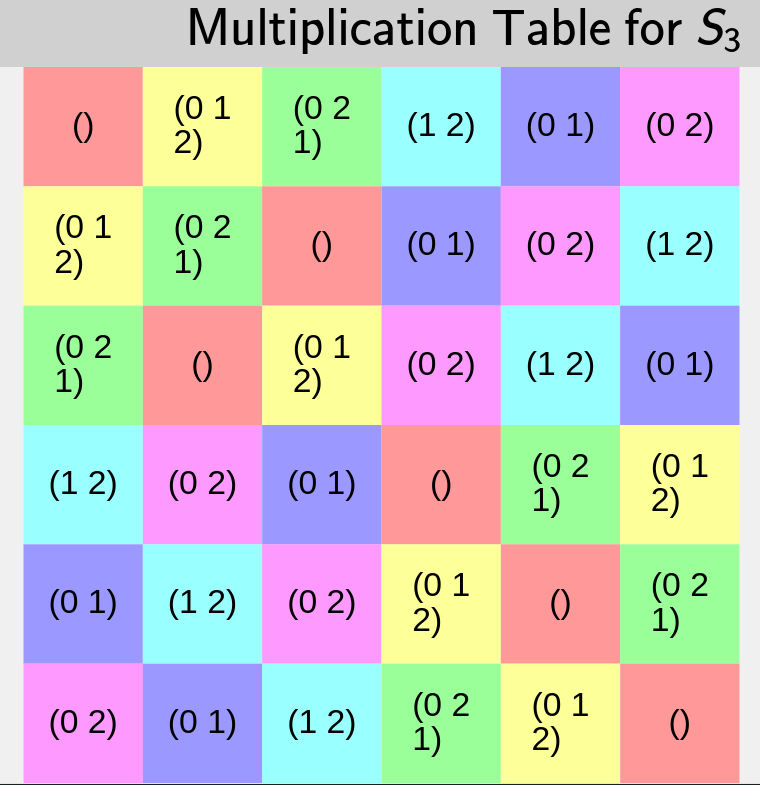
\includegraphics[scale=0.25]{images/group_gap_01.png}
\end{figure}
    
This has to read as "row times column"; as an example consider the second row (holding the permutation $(0,1,2)$) and third column (holding the permutation $(0,2,1)$). Let's "multiply" these two permutations; i.e. we first apply $(0,2,1)$ followed by $(0,1,2)$:

\begin{itemize}
    \item If we have a $0$, the permutation $(0,2,1)$ maps it into a $2$ which the second permutation $(0,1,2)$ maps it into a $0$. So - all in all - nothing happens.
    \item If we have a $1$, the permutation $(0,2,1)$ maps it into a $0$ which the second permutation $(0,1,2)$ maps it into a $1$. So - all in all - nothing happens.
    \item If we have a $2$, the permutation $(0,2,1)$ maps it into a $1$ which the second permutation $(0,1,2)$ maps it into a $2$. So - again - nothing happens.
\end{itemize}

All in all, the multiplication of these two permutations yields the identity element denoted as $e$ or $()$.

For the fun of it, let's try another one: row $4$ times column $3$. We have

\bee
(1,2) (0,2,1) = (0,1)
\eee

To show that this is a non-Abelian group, we apply the permutations the other way round. We obtain

\bee
(0,2,1) (1,2) = (0,2)
\eee

which is something different. These two results can also be found in the multiplication table above at the corresponding locations.

We can perform the multiplication using GAP as well; we need to be careful not to use zeros, however. Multiplication $(0,1,2)(0,2,1)$ becomes

\begin{verbatim}
    gap> (1,2,3)*(1,3,2);
    ()
\end{verbatim}

In a similar spirit, we have

\begin{verbatim}
    gap> (1,3,2)*(2,3);
    (1,2)
    gap> (2,3)*(1,3,2);
    (1,3)
\end{verbatim}

which correspond to $(0,1)$ and $(0,2)$, respectively.

Of course, GAP knows about the symmetric group $S_3$. We can construct the group and display its elements as follows.

\begin{verbatim}
    gap> S3 := SymmetricGroup(3);
    Sym( [ 1 .. 3 ] )
    gap> e := Elements(S3);
    [ (), (2,3), (1,2), (1,2,3), (1,3,2), (1,3) ]
\end{verbatim}

GAP allows to calculate the multiplication table as follows.

\begin{verbatim}
    gap> table:=Display(MultiplicationTable(G));
    [ [  1,  2,  3,  4,  5,  6 ],
      [  2,  1,  4,  3,  6,  5 ],
      [  3,  5,  1,  6,  2,  4 ],
      [  4,  6,  2,  5,  1,  3 ],
      [  5,  3,  6,  1,  4,  2 ],
      [  6,  4,  5,  2,  3,  1 ] ]
\end{verbatim}

The table contains indices to the group elements stored in variable \verb e above. As an example, let's perform \verb (1,3,2)*(2,3) : The permutation \verb (1,3,2)  is located at index $5$ and the permutation \verb (2,3)  is located at index $2$.  Looking at row $5$, column $2$ of the multiplication table we read off index $3$ (we could have used \verb table[5,2] ) which corresponds to $(1,2)$. This corresponds to the result from above where we directly calculated the product of the two permutations.

We can use GAP to simplify the process and output permutations right away.

\begin{verbatim}
    S3 := SymmetricGroup(3);
    e := Elements(S3);
    n:=Order(S3);

    M:=MultiplicationTable(S3);

    for i in [1..n] do
        for j in [1..n] do
        ind := M[i][j];
        Print(e[ind], "   ");
        od;
    Print("\n");
    od;
    Print("\n");
\end{verbatim}

This yields the following result (slightly reformatted for easier reading)

\begin{verbatim}
       ()    (2,3)      (1,2)    (1,2,3)   (1,3,2)     (1,3)
    (2,3)       ()    (1,2,3)      (1,2)     (1,3)   (1,3,2)
    (1,2)  (1,3,2)         ()      (1,3)     (2,3)   (1,2,3)
  (1,2,3)    (1,3)      (2,3)    (1,3,2)        ()     (1,2)
  (1,3,2)    (1,2)      (1,3)         ()   (1,2,3)     (2,3)
    (1,3)  (1,2,3)    (1,3,2)      (2,3)     (1,2)        ()
\end{verbatim}

We can obtain the same results as from the previous calculations.

Last but not least, let's obtain the generators of $S_3$ using

\begin{verbatim}
    gap> GeneratorsOfGroup(S3);
    [ (1,2,3), (1,2) ]
\end{verbatim}

By taking various products of the generators, we can obtain all (other) group elements (that's the way generators are defined); in our case as follows.

\begin{verbatim}
    gap> (1,2)*(1,2);
    ()
    gap> (1,2,3)*(1,2,3);
    (1,3,2)
    gap> (1,2,3)*(1,2);
    (2,3)
    gap> (1,2)*(1,2,3);
    (1,3)
\end{verbatim}


\subsection{Subgroups of $S_3$}

We can use \verb|AllSubgroups| to list all subgroups of a group; however, this usually produces \emph{a lot} of entries.

\begin{verbatim}
    gap> sg := AllSubgroups(S3);
    [ Group(()), Group([ (2,3) ]), Group([ (1,2) ]), Group([ (1,3) ]), 
    Group([ (1,2,3) ]), Group([ (1,2,3), (2,3) ]) ]
\end{verbatim}

Trivially, the empty group (\verb sg[1]  and the group itself \verb sg[6] ) are subgroups. However, there are some more interesting subgroups: The three subgroups $(1,2)$, $(2,3)$, and $(1,3)$ which are all isomorphic, and the subgroup $(1,2,3)$.

\paragraph{Group $(1,2)$ and Isomorphisms.} For the three isomorphic groups, we can do the following:

\begin{verbatim}
    gap> sg1 := sg[2];
    Group([ (2,3) ])
    gap> sg2 := sg[3];
    Group([ (1,2) ])
    gap> sg3 := sg[4];
    Group([ (1,3) ])
    gap> IdGroup(sg1) = IdGroup(sg2);
    true
    gap> IdGroup(sg1) = IdGroup(sg3);
    true
\end{verbatim}

Further analysis shows that the group has order $2$, is an Abelian group and a cyclic one.

\begin{verbatim}
    gap> Order(sg1);
    2
    gap> IsAbelian(sg1);
    true
    gap> IsCyclic(sg1);
    true
\end{verbatim}

Since the group is cyclic, it has one generator and further rinspection shows that it is isomorphic to \emph{C2}.

\begin{verbatim}
    gap> GeneratorsOfGroup(sg1);
    [ (2,3) ]
    gap> StructureDescription(sg1);
    "C2"
\end{verbatim}

By slightly adapting our previous multiplication table function, we obtain a multiplication table for this group as

\begin{verbatim}
    gap> ShowMulTable(sg1);
    ()   (2,3)   
    (2,3)   ()   
\end{verbatim}

\paragraph{Group $(1,2,3)$.} Let's see what's this for a group. We have

\begin{verbatim}
    gap> s:=sg[5];
    Group([ (1,2,3) ])
    gap> Order(s);
    3
    gap> IsAbelian(s);
    true
    gap> IsCyclic(s);
    true
    gap> StructureDescription(s);
    "C3"
\end{verbatim}

For the multiplication table we obtain

\begin{verbatim}
    gap> ShowMulTable(s);
    ()        (1,2,3)   (1,3,2)   
    (1,2,3)   (1,3,2)        ()   
    (1,3,2)        ()   (1,2,3)   
\end{verbatim}


%%% Local Variables:
%%% mode: latex
%%% TeX-master: "journal"
%%% End:
